% Compile with pdfLaTeX.
% Landscape version corresponding to the revised portrait template.
% Font matching is intentionally relaxed for this version.

\documentclass[a4paper,landscape]{article}

% Scroll down to line 74

% Minimal external packages:
\usepackage[a4paper,landscape,left=18mm,right=18mm,top=18mm,bottom=18mm]{geometry}
\usepackage{graphicx}
\usepackage{xcolor}
\usepackage{lipsum}
\usepackage{array}
\usepackage[T1]{fontenc}
\usepackage[sfdefault]{roboto}
\usepackage[
    colorlinks=true,
    urlcolor=blue,
    linkcolor=black,
    citecolor=blue
]{hyperref}

\pagestyle{empty}
\setlength{\parindent}{0pt}
\setlength{\parskip}{0pt}
\setlength{\tabcolsep}{0pt}
\definecolor{topicblue}{HTML}{2F5597}

% Lengths - specifications for template fonts, appearance
\newlength{\HeaderSize}
\setlength{\HeaderSize}{24pt}
\newlength{\HeaderSizeBaseline}
\setlength{\HeaderSizeBaseline}{28.8pt}

\newlength{\SectionSize}
\setlength{\SectionSize}{16pt}
\newlength{\SectionSizeBaseline}
\setlength{\SectionSizeBaseline}{1.2\SectionSize}

\newlength{\TextSize}
\setlength{\TextSize}{14pt}
\newlength{\TextSizeBaseline}
\setlength{\TextSizeBaseline}{1.3\TextSize}

\newlength{\CaptionSize}
\setlength{\CaptionSize}{12pt}
\newlength{\CaptionSizeBaseline}
\setlength{\CaptionSizeBaseline}{1.2\CaptionSize}

\newlength{\RefSize}
\setlength{\RefSize}{12pt}
\newlength{\RefSizeBaseline}
\setlength{\RefSizeBaseline}{1.4\RefSize}

\newlength{\vskipHeader}
\setlength{\vskipHeader}{8.0mm}
\newlength{\vskipSection}
\setlength{\vskipSection}{4.0mm}
\newlength{\vskipText}
\setlength{\vskipText}{2.0mm}
\newlength{\vskipImage}
\setlength{\vskipImage}{16.0mm}

% Landscape geometry.
% The left panel is square; the right panel uses the remaining width.
\newlength{\LeftPanel}
\setlength{\LeftPanel}{164mm}
\newlength{\PanelGap}
\setlength{\PanelGap}{18mm}
\newlength{\RightPanel}
\setlength{\RightPanel}{79mm}

% Do not change anything above this line!

\begin{document}
\noindent
\begin{tabular}{@{}p{\LeftPanel}@{\hspace{\PanelGap}}p{\RightPanel}@{}}

% ======================= LEFT SQUARE =======================
\parbox[t][\LeftPanel][t]{\LeftPanel}{%

% High page header
\begin{center}
  {\fontsize{\HeaderSize}{\HeaderSizeBaseline}\selectfont\color{topicblue}%
  %
  % Agnese will modify this; For now write your name and number your projects with 1 and 2
   Project Topic:\hspace{9mm} (Xinwen 1)} 
\end{center}

\vspace{\vskipHeader}

% Main title
{\fontsize{\SectionSize}{\SectionSizeBaseline}\selectfont\bfseries 
%
% Title
Optimizing Collective Escape in Predator–Prey Systems
\par}
\vspace{\vskipSection}

% Abstract / project description --> adjust accordingly
{\fontsize{\TextSize}{\TextSizeBaseline}\selectfont
%
% Intro+Motivation
Collective motion is common in prey species such as fish, birds, and insects, where coordinated group behavior can reduce predation risk. However, stronger coordination is not always better: while cohesive groups may transmit information quickly, they may also lose maneuverability or become easier targets. In this project, students will develop a predator–prey model in which prey follow Vicsek-inspired rules with alignment, cohesion, repulsion, limited perception, and predator avoidance, while predators may use different pursuit strategies [1, 2].
\par

\vspace{\vskipText}
% In this project
The main goal is to determine which collective movement strategies maximize prey survival. You will formulate your own optimization problem by varying behavioral parameters, group size, sensory information, environmental conditions, or predator strategies, and evaluate performance using measures such as survival probability, capture rate, response time, and group fragmentation. 
\par
}

\vfill
\vspace{\vskipSection}
% References are entered manually. No .bib file / BibTeX / biblatex.
{\fontsize{\SectionSize}{\SectionSizeBaseline}\selectfont\bfseries References:\par}
\vspace{\vskipSection}

{\fontsize{\RefSize}{\RefSizeBaseline}\selectfont
% 
% Reference 1
[1] Vicsek, T., et al.
\textit{Novel Type of Phase Transition in a System of Self-Driven Particles}, Phys. Rev. Lett. \textbf{75}, 1226–1229 (1995).\\
\href{https://doi.org/10.1103/PhysRevLett.75.1226}{https://doi.org/10.1103/PhysRevLett.75.1226} 
\par
% 
[2] Bartashevich, P., et al.
\textit{Collective anti-predator escape manoeuvres through optimal attack and avoidance strategies}, Commun. Biol. \textbf{7}, 1586 (2024).\\
\href{https://doi.org/10.1038/s42003-024-07267-2}{https://doi.org/10.1038/s42003-024-07267-2} 
% Add Reference 2 (if needed)
\par
% 
% Add a Reference 3 (if needed)
\par
}
\vspace{\vskipText}
}% end left square

&

% ======================= RIGHT COLUMN =======================
\parbox[t][\LeftPanel][c]{\RightPanel}{%
\centering
%
% Representative image + caption. 
\begin{tabular}{@{}c@{}}
%
% Image
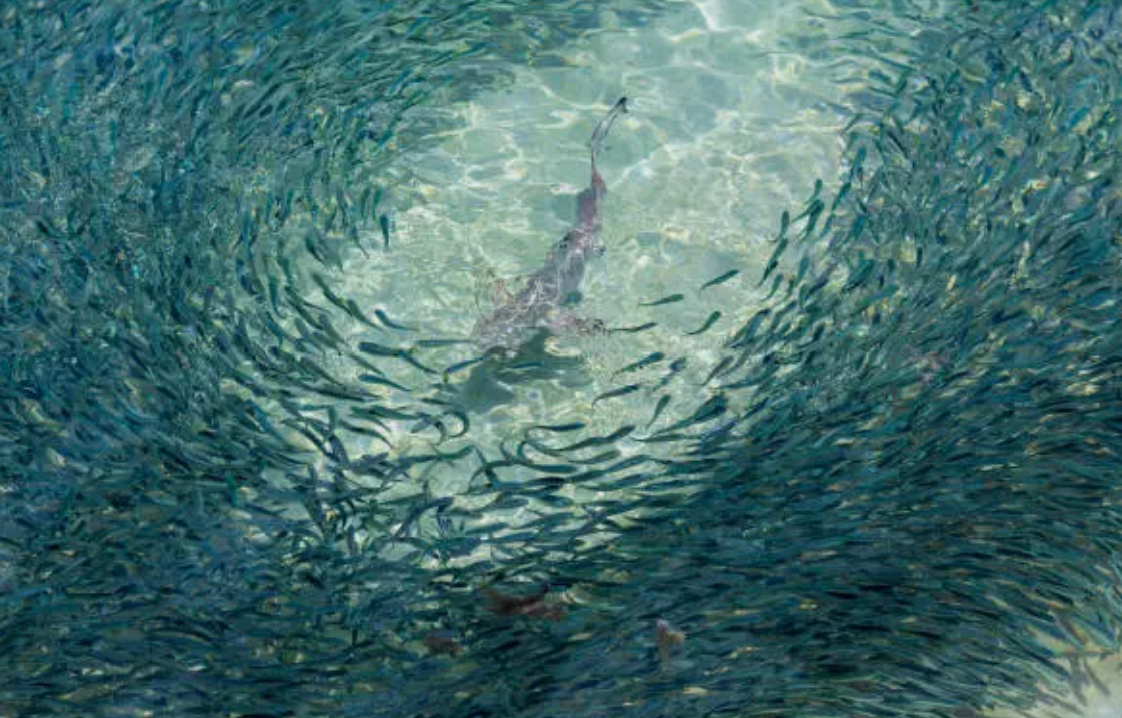
\includegraphics[width=\RightPanel]{shark.png}\\[\vskipSection] % name of the image 
\parbox{\RightPanel}{%
\fontsize{\CaptionSize}{\CaptionSizeBaseline}\selectfont
\textbf{Fig.1}\quad 
% 
% Title of the image (bold)
\textbf{Photo of gray shark surrounded with fishes} 
% 
% Body of the image caption.
Self-organized collective behavior is widespread in living systems, such as schools of fish. By coordinating their motion, fish can respond collectively to threats, improving the chances of avoiding predators such as gray sharks.
%
% Credits.
\textit{Photo by Tony Studio on} 
\href{https://unsplash.com/photos/gray-shark-surrounded-with-fishes-qSR0KbeNbtk}{iStock} 
}
\end{tabular}
}% end right column

\end{tabular}
\end{document}
